\doclearpage
\section{Pre-Filtering Optimization}

In \cref{sec:piop-for-pattern-matching} we presented a PIOP for pattern matching that is proven secure and ready to be deployed. Although \cref{piop:multi-char-pattern-matching} proves what is conceptually a simple filter, it operates on the full character-level machinery of the string arithmetization and is therefore expensive. This motivates us to shrink the string columns fed into it as much as possible.

To this end, we borrow the \emph{fingerprinting} technique from the database literature, where it was introduced~\cite{string_fingerprint} as a fast pre-filter for query execution: it cheaply discards \emph{true negatives}, the rows that certainly do not match the pattern, while possibly retaining \emph{false positives}, rows that survive the filter but do not actually match. Once most true negatives are gone, the surviving column is small enough that an exact but expensive pattern-matching protocol can affordably remove the remaining false positives.

Although fingerprinting was originally proposed to speed up the \emph{execution} of pattern matching, we find that it speeds up its \emph{verification} just as effectively. Before presenting the verification mechanism, we first describe how fingerprint-based pre-filtering works.

\subsection{Pre-Filtering via Fingerprinting}

The idea of fingerprinting is to replace the full representation of a string with a handful of \emph{bins}, each bin holding a single bit that is $1$ if and only if the string satisfies a fixed property. The fingerprint of a string is the vector of its bin values.

For example, suppose we have $m=4$ bins, where bin $i\in\{1,2,3,4\}$ is computed by its own predicate $\mathsf{fp}_i: \mathsf{Strings} \to \{0,1\}$ defined as follows:
\begin{align*}
 &\mathsf{fp}_1(\mathsf{s}) = \begin{cases}
  1 & \text{if $\mathsf{s}$ contains `a', `b', or `c'}\\
  0 & \text{otherwise}
 \end{cases}
 \qquad
 &\mathsf{fp}_2(\mathsf{s}) = \begin{cases}
  1 & \text{if $\mathsf{s}$ contains any of `d', `e', \dots, `l'}\\
  0 & \text{otherwise}
 \end{cases}
 \\
 &\mathsf{fp}_3(\mathsf{s}) = \begin{cases}
  1 & \text{if $\mathsf{s}$ contains `m' or `n'}\\
  0 & \text{otherwise}
 \end{cases}
 \qquad
 &\mathsf{fp}_4(\mathsf{s}) = \begin{cases}
  1 & \text{if $\mathsf{s}$ contains any of `o', `p', \dots, `z'}\\
  0 & \text{otherwise}
 \end{cases}
\end{align*}

Now suppose we want to evaluate the filter \texttt{\%dar\%} on the strings \texttt{darling}, \texttt{zebra}, and \texttt{lemon}. Fingerprinting the pattern's literal \texttt{dar} and the three strings yields
\begin{equation*}
 \texttt{dar}\to 1101,\qquad \texttt{darling} \to 1111,\qquad \texttt{zebra} \to 1101,\qquad \texttt{lemon}\to 0111.
\end{equation*}

A string can match \texttt{\%dar\%} only if it contains every character of \texttt{dar}, so every bin that is active in the pattern's fingerprint must also be active in the string's fingerprint. The first bin is active in the pattern but inactive in \texttt{lemon}: \texttt{lemon} contains none of `a', `b', `c', so it cannot contain \texttt{dar} and is discarded immediately. Both \texttt{darling} and \texttt{zebra}, on the other hand, activate every bin that the pattern does, so both survive the filter. Of these, \texttt{darling} is a genuine match, whereas \texttt{zebra} does not satisfy the predicate and is a \emph{false positive} that only the exact protocol can remove.

\subsection{A PIOP for Pre-Filtering}
\label{sec:prefilter-piop}

\parhead{Fingerprints as integers} We pack the $m$ bins of a fingerprint into a single field element by reading the bin vector as an $m$-bit integer, bin $1$ being the most significant bit:
\begin{equation*}
  \mathsf{fp}(\mathsf{s}) := \sum_{i=1}^{m} 2^{m-i}\,\mathsf{fp}_i(\mathsf{s}) \in [0, 2^m-1].
\end{equation*}
A pattern $\zeta$ is fingerprinted through its literal characters only: the wild-cards are dropped and the characters of all factors are pooled, so $\mathsf{fp}(\zeta)$ is the fingerprint of the string obtained by concatenating the factors. Throughout this subsection we write $\phi := \mathsf{fp}(\zeta)$ for this public constant. Since every character of $\zeta$ must appear in any string that matches it, the subset condition of the previous subsection is precisely the bitwise identity
\begin{equation*}
  \mathsf{fp}(\mathsf{s}) \land \phi = \phi,
\end{equation*}
where $\land$ denotes bitwise AND. This is the operation that the Bitwise AND check of \cref{sec:bitwise-and} proves, and it is the sole non-linear ingredient of the protocol below.

\parhead{The fingerprint column} For the verifier to benefit from pre-filtering, the fingerprints must be available without touching the character-level columns. We therefore extend the string arithmetization of \cref{sec:string-arith} with one more string-level auxiliary column, the \emph{fingerprint column} $\mathsf{fp}$, with $\mathsf{fp}[i] = \mathsf{fp}(\col[i])$ the $m$-bit fingerprint of the $i$-th string. Like the length column $\mathsf{l}$, it is computed once at ingestion and then carried along by the consistency-checking protocols of \cref{sec:consistency-checking}: a data-preserving update inherits it unchanged, and a domain-preserving update copies it from the source row through the same lookup that transfers $\mathsf{h}$ and $\mathsf{l}$. Hence, by the time a pattern-matching query arrives, $\mathsf{fp}$ is trusted.

\parhead{The relation} Pre-filtering is itself a data-preserving update: the prover freshly materializes the activators $\mathsf{a'}$ and $\mathsf{char\text{-}act'}$, keeping exactly the active strings whose fingerprint passes the subset test, and every other column is inherited. We package this as the relation
\begin{equation*}
\NPRelation_{\mathsf{PreFilter}} = \left\{
\begin{aligned}
  & \NPInstance = (m, \phi),\; \\
  & \NPInstancey = (\Oracle{\MLE{\mathsf{fp}}}, \Oracle{\MLE{\mathsf{a}}}, \Oracle{\MLE{\mathsf{char\text{-}act}}}, \Oracle{\MLE{\mathsf{a'}}}, \Oracle{\MLE{\mathsf{char\text{-}act'}}}),\; \\
  & \NPWitness = (\mathsf{fp}, \mathsf{a}, \mathsf{char\text{-}act}, \mathsf{a'}, \mathsf{char\text{-}act'})
\end{aligned}
   \;\middle|\;
    \begin{aligned}
   \mathsf{a'}[i] = 1 \iff \bigl(\mathsf{a}[i] = 1 \ \text{and}\ \mathsf{fp}[i] \land \phi = \phi\bigr) \\
    \mathsf{char\text{-}act'}[j] = \mathsf{a'}[i]\ \forall\text{ char } j \text{ of string } i
    \end{aligned}
\right\}.
\end{equation*}
The relation mirrors $\NPRelation_{\mathsf{LenFilter}}$ of \cref{sec:length-filtering}, with the length threshold replaced by the fingerprint test; both are filters that may only switch strings off.

\parhead{The protocol} The first two steps are the standard ones for any filter: the new activator pair must be consistent (\cref{piop:data-preserving-update-check}), and no inactive string may be revived (a zerocheck on $\mathsf{a'}\mult(1-\mathsf{a})$). The remaining steps enforce the fingerprint test. The prover sends the \emph{masked column} $\mathsf{g} := \mathsf{fp} \land \phi$, obtained by AND-ing every fingerprint with the pattern fingerprint, and the parties certify it with the Bitwise AND check applied to $\mathsf{fp}$, the constant column $\phi\mult\mathbf{1}$, and $\mathsf{g}$; the constant column needs no oracle, as its multilinear extension is the constant $\phi$, which the verifier evaluates by itself. Once $\mathsf{g}$ is certified, the test $\mathsf{fp}[i] \land \phi = \phi$ becomes the equality $\mathsf{g}[i] = \phi$, and it is here that the AND structure pays off a second time: $\mathsf{g}[i]$ is a sub-mask of $\phi$, so as an integer $\mathsf{g}[i] \leq \phi$ always holds, with equality exactly for the strings that pass. Consequently $\mathsf{g} - \phi$ is zero on the survivors and strictly negative on every string that fails, and the verdict splits into the same two one-sided checks as length filtering: a zerocheck on $\mathsf{a'}\mult(\mathsf{g}-\phi)$ rules out false positives (no kept string fails the test), and a $\mathsf{Neg}$ sign check on $\mathsf{g}-\phi$ activated by $\mathsf{a}\mult(1-\mathsf{a'})$ rules out false negatives (every dropped string genuinely fails). The sign check needs width $m$, since $|\mathsf{g}[i]-\phi| < 2^m$.

\begin{DefinePIOP}{Pre-Filtering Check}{prefilter}
  \emph{Inputs:} $\Oracle{\MLE{\mathsf{fp}}}, \Oracle{\MLE{\mathsf{a}}}, \Oracle{\MLE{\mathsf{char\text{-}act}}}, \Oracle{\MLE{\mathsf{a'}}}, \Oracle{\MLE{\mathsf{char\text{-}act'}}}, \Oracle{\MLE{\mathsf{orig\text{-}ind}}}, \Oracle{\MLE{\mathsf{ind}}}, \Oracle{\MLE{\mathsf{l}}}$, bin count $m$, pattern fingerprint $\phi$.
  \begin{enumerate}[nosep]
    \item (\textit{Activator Update Validity}) $\PIOPProver$ and $\PIOPVerifier$ invoke \cref{piop:data-preserving-update-check} on $(\mathsf{char\text{-}act'}, \mathsf{a'}, \mathsf{orig\text{-}ind},\allowbreak \mathsf{ind}, \mathsf{l})$.
    \item (\textit{Containment}) $\PIOPProver$ and $\PIOPVerifier$ invoke \cref{piop:zerocheck} on the column $\mathsf{a'}\mult(1-\mathsf{a})$.
    \item (\textit{Masking}) $\PIOPProver$ computes the masked column $\mathsf{g} := \mathsf{fp} \land \phi$ and sends $\Oracle{\MLE{\mathsf{g}}}$ to $\PIOPVerifier$. The parties invoke \cref{piop:bitwise-and} on $(\mathsf{fp}, \phi\mult\mathbf{1}, \mathsf{g})$ with bit-width $n = m$.
    \item (\textit{False Positive check}) $\PIOPProver$ and $\PIOPVerifier$ invoke \cref{piop:zerocheck} on the column $\mathsf{a'}\mult(\mathsf{g}-\phi)$.
    \item (\textit{False Negative check}) $\PIOPProver$ and $\PIOPVerifier$ invoke the $\mathsf{Neg}$ \cref{piop:sign-check} on the column $(\mathsf{a}\mult(1-\mathsf{a'}),\ \mathsf{g}-\phi)$ with width $m$.
  \end{enumerate}
\end{DefinePIOP}

\parhead{Cost} Every step of \cref{piop:prefilter} runs over string-level columns of length $N$, except the activator-validity check, which is shared with any filter; in particular, the character column is never opened, which is exactly what makes pre-filtering cheap relative to \cref{piop:multi-char-pattern-matching}. After pre-filtering, the prover compacts the survivors into a fresh, smaller column via \cref{piop:full-str-valid} and runs the exact pattern-matching protocol on that column alone, where it removes the remaining false positives. Note also that one operand of the AND is the public constant $\phi$, so the two-operand truth table of \cref{piop:bitwise-and}, which has $2^{2m}$ rows, can be replaced by the $2^m$-row table $(\idx_m, \idx_m \land \phi)$, whose second component has the linear multilinear extension $\sum_{i:\ \text{bit } i \text{ of } \phi \text{ is set}} 2^{m-1-i} X_i$; we present the protocol with the general check for uniformity.

\subsection{Bitwise AND}
\label{sec:bitwise-and}
The \emph{Bitwise AND check} takes three columns $\col_1, \col_2, \col_3$ containing $n$-bit values and proves that every entry of $\col_3$ is the bitwise AND of the corresponding entries in $\col_1$ and $\col_2$. We package this as the relation
\begin{displaymath}
\NPRelation_{\mathsf{BitwiseAND}} = \left\{\,
  \NPInstance = n,\;
  \NPInstancey = (\Oracle{\MLE{\col_1}}, \Oracle{\MLE{\col_2}}, \Oracle{\MLE{\col_3}}),\;
  \NPWitness = (\col_1, \col_2, \col_3)
  \;\middle|\;
    \forall i,\, \col_3[i] = \col_1[i] \land \col_2[i]
\,\right\}.
\end{displaymath}

\ifsp
%% Single-column (IEEE) variant: columns laid out horizontally as rows.
\begin{figure}[tp]
\centering
\resizebox{\columnwidth}{!}{%
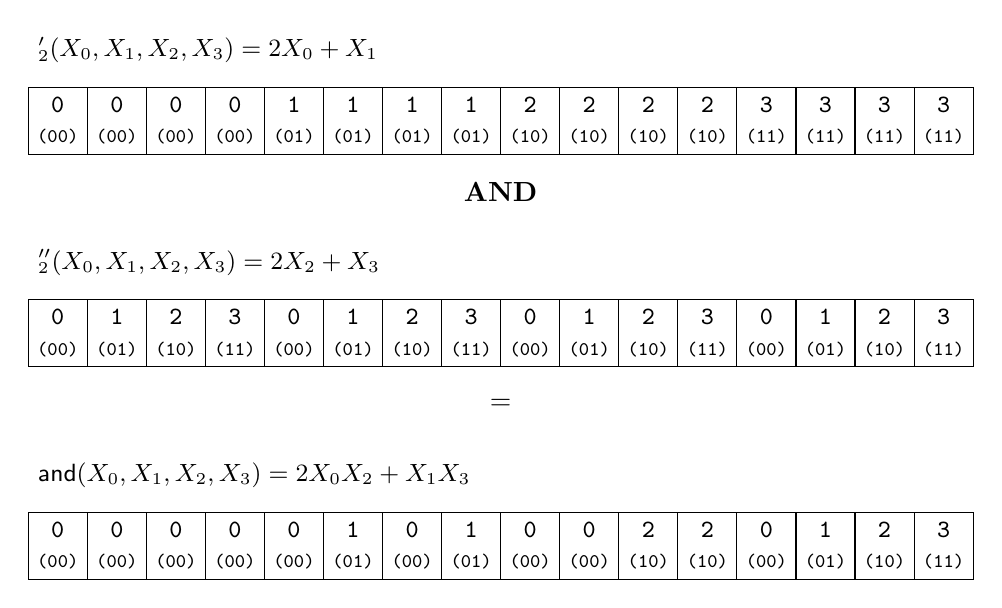
\begin{tikzpicture}[
  cell/.style={draw, align=center, minimum width=0.75cm, minimum height=0.85cm, font=\ttfamily\small, inner sep=1pt},
  plab/.style={anchor=west, font=\small},
  op/.style={font=\bfseries}
]
\def\cellW{0.75}
% --- column 1 ---
\node[plab] at (-0.375, 0) {$\idx'_2(X_0,X_1,X_2,X_3) = 2X_0 + X_1$};
\foreach \val/\bin [count=\i from 0] in
  {0/00,0/00,0/00,0/00,1/01,1/01,1/01,1/01,2/10,2/10,2/10,2/10,3/11,3/11,3/11,3/11}
  {\node[cell] at (\cellW*\i, -0.9) {\val\\{\scriptsize(\bin)}};}
% --- AND ---
\node[op] at (\cellW*7.5, -1.8) {AND};
% --- column 2 ---
\node[plab] at (-0.375, -2.7) {$\idx''_2(X_0,X_1,X_2,X_3) = 2X_2 + X_3$};
\foreach \val/\bin [count=\i from 0] in
  {0/00,1/01,2/10,3/11,0/00,1/01,2/10,3/11,0/00,1/01,2/10,3/11,0/00,1/01,2/10,3/11}
  {\node[cell] at (\cellW*\i, -3.6) {\val\\{\scriptsize(\bin)}};}
% --- = ---
\node[op] at (\cellW*7.5, -4.5) {$=$};
% --- column 3 ---
\node[plab] at (-0.375, -5.4) {$\MLE{\mathsf{and}}(X_0,X_1,X_2,X_3) = 2X_0X_2 + X_1X_3$};
\foreach \val/\bin [count=\i from 0] in
  {0/00,0/00,0/00,0/00,0/00,1/01,0/00,1/01,0/00,0/00,2/10,2/10,0/00,1/01,2/10,3/11}
  {\node[cell] at (\cellW*\i, -6.3) {\val\\{\scriptsize(\bin)}};}
\end{tikzpicture}%
}
\caption{The arithmetized truth-table for the bitwise AND function on $n=2$ bit inputs, with the three columns laid out as rows.}
\label{fig:bitwise-and-tt}
\end{figure}
\else
\begin{figure}[h]
\centering
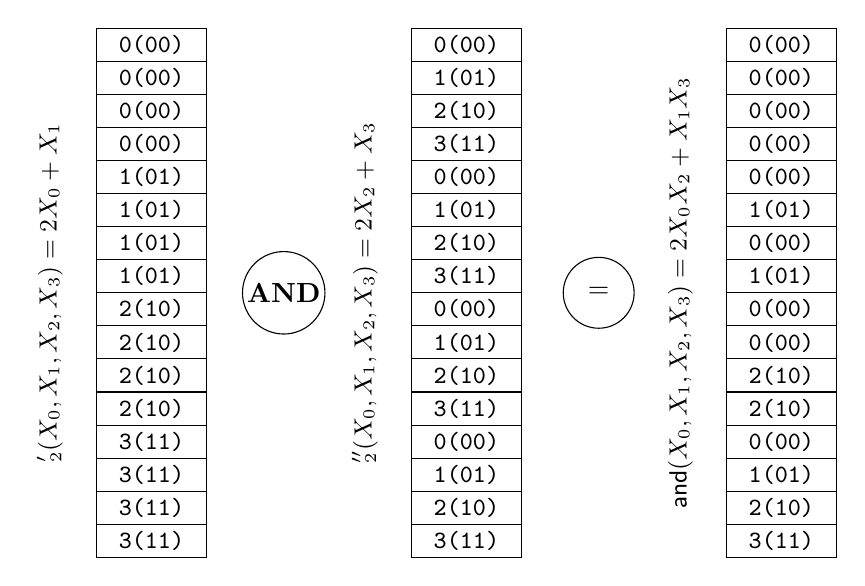
\begin{tikzpicture}[
  cell/.style={draw, minimum width=1.4cm, minimum height=0.42cm, font=\ttfamily\small, inner sep=1pt},
  op/.style={draw, circle, minimum size=0.9cm, font=\bfseries, inner sep=1pt, fill=white},
  collabel/.style={rotate=90, anchor=south, font=\small}
]
\def\cellH{0.42}
\def\colSep{4.0}
\foreach \v [count=\i from 0] in
  {0(00),0(00),0(00),0(00),1(01),1(01),1(01),1(01),2(10),2(10),2(10),2(10),3(11),3(11),3(11),3(11)}
  {\node[cell] (a\i) at (0, -\cellH*\i) {\v};}
\foreach \v [count=\i from 0] in
  {0(00),1(01),2(10),3(11),0(00),1(01),2(10),3(11),0(00),1(01),2(10),3(11),0(00),1(01),2(10),3(11)}
  {\node[cell] (b\i) at (\colSep, -\cellH*\i) {\v};}
\foreach \v [count=\i from 0] in
  {0(00),0(00),0(00),0(00),0(00),1(01),0(00),1(01),0(00),0(00),2(10),2(10),0(00),1(01),2(10),3(11)}
  {\node[cell] (c\i) at (2*\colSep, -\cellH*\i) {\v};}
\node[op] at (0.42*\colSep, -\cellH*7.5) {AND};
\node[op] at (1.42*\colSep, -\cellH*7.5) {$=$};
\node[collabel] at (-1.0, -\cellH*7.5) {$\idx'_2(X_0,X_1,X_2,X_3) = 2X_0 + X_1$};
\node[collabel] at (\colSep-1.0, -\cellH*7.5) {$\idx''_2(X_0,X_1,X_2,X_3) = 2X_2 + X_3$};
\node[collabel] at (2*\colSep-1.0, -\cellH*7.5) {$\MLE{\mathsf{and}}(X_0,X_1,X_2,X_3) = 2X_0X_2+X_1X_3$};
\end{tikzpicture}
\caption{The arithmetized truth-table for the bitwise AND function on n=2 bit inputs.}
\label{fig:bitwise-and-tt}
\end{figure}
\fi

To convince the verifier that each row of $\col_3$ is the bitwise AND of the corresponding rows of $\col_1$ and $\col_2$, the prover will convince the verifier that the concatenated rows of $\col_1, \col_2, \col_3$ can be looked up in a truth table encoding the bitwise AND function. More concretely,
\begin{DefinePIOP}{BitwiseAND}{bitwise-and}
    \begin{enumerate}[nosep]
        \item $\PIOPProver$ and $\PIOPVerifier$ invoke \cref{piop:range-check} on each of the three columns to check that they are all $n$-bit.
        \item $\PIOPVerifier$ samples three random field elements $r_1, r_2,r_3$ and sends them to $\PIOPProver$.
        \item $\PIOPProver$ and $\PIOPVerifier$ invoke \cref{piop:lookup-check} to check that the concatenated column $\col' = r_1\col_1 + r_2\col_2 + r_3\col_3$ can be looked up in the column $\col'' = r_1\idx'_n+r_2\idx''_n+r_3\MLE{o}$ where
        \begin{align*}
            \idx'_n(X_0,\ldots,X_{n-1}) &= \sum_{i=0}^{n-1} 2^{n-1-i} X_i, \\
            \idx''_n(X_0,\ldots,X_{n-1}) &= \sum_{i=0}^{n-1} 2^{n-1-i} X_{n+i}, \\
            \MLE{\mathsf{and}}(X_0,\ldots,X_{2n-1}) &= \sum_{i=0}^{n-1} 2^{n-1-i} X_iX_{n+i}.
        \end{align*}
    \end{enumerate}
\end{DefinePIOP}
